%-----------------------------------------------------------------------------------------------------------------------------------------------%
%	The MIT License (MIT)
%
%	Copyright (c) 2019 Jan Küster
%
%	Permission is hereby granted, free of charge, to any person obtaining a copy
%	of this software and associated documentation files (the "Software"), to deal
%	in the Software without restriction, including without limitation the rights
%	to use, copy, modify, merge, publish, distribute, sublicense, and/or sell
%	copies of the Software, and to permit persons to whom the Software is
%	furnished to do so, subject to the following conditions:
%	
%	THE SOFTWARE IS PROVIDED "AS IS", WITHOUT WARRANTY OF ANY KIND, EXPRESS OR
%	IMPLIED, INCLUDING BUT NOT LIMITED TO THE WARRANTIES OF MERCHANTABILITY,
%	FITNESS FOR A PARTICULAR PURPOSE AND NONINFRINGEMENT. IN NO EVENT SHALL THE
%	AUTHORS OR COPYRIGHT HOLDERS BE LIABLE FOR ANY CLAIM, DAMAGES OR OTHER
%	LIABILITY, WHETHER IN AN ACTION OF CONTRACT, TORT OR OTHERWISE, ARISING FROM,
%	OUT OF OR IN CONNECTION WITH THE SOFTWARE OR THE USE OR OTHER DEALINGS IN
%	THE SOFTWARE.
%	
%
%-----------------------------------------------------------------------------------------------------------------------------------------------%


%============================================================================%
%
%	DOCUMENT DEFINITION
%
%============================================================================%

%we use article class because we want to fully customize the page and don't use a cv template

\documentclass[10pt,A4]{article}

%----------------------------------------------------------------------------------------
%	ENCODING
%----------------------------------------------------------------------------------------

% we use utf8 since we want to build from any machine
 

%----------------------------------------------------------------------------------------
%	LOGIC
%----------------------------------------------------------------------------------------

% provides \isempty test
\usepackage{xstring, xifthen}

%----------------------------------------------------------------------------------------
%	FONT BASICS
%----------------------------------------------------------------------------------------

% some tex-live fonts - choose your own

%\usepackage[defaultsans]{droidsans}
%\usepackage[default]{comfortaa}
%\usepackage{cmbright}
 
%\usepackage{fetamont}
%\usepackage[default]{gillius}
%\usepackage[light,math]{iwona}
%\usepackage[thin]{roboto} 

% set font default
%\renewcommand*\familydefault{\sfdefault} 	
%\usepackage[T1]{fontenc}


\usepackage{fontspec} 					                 % for loading fonts



  \setmainfont{SourceSansPro-Light}[
Path = fonts/,
BoldFont = SourceSansPro-Regular,
ItalicFont = SourceSansPro-LightIt]

% more font size definitions
\usepackage{moresize}

%----------------------------------------------------------------------------------------
%	FONT AWESOME ICONS
%---------------------------------------------------------------------------------------- 

% include the fontawesome icon set
\usepackage{fontawesome}

% use to vertically center content
% credits to: http://tex.stackexchange.com/questions/7219/how-to-vertically-center-two-images-next-to-each-other
\newcommand{\vcenteredinclude}[1]{\begingroup
\setbox0=\hbox{\includegraphics{#1}}%
\parbox{\wd0}{\box0}\endgroup}

% use to vertically center content
% credits to: http://tex.stackexchange.com/questions/7219/how-to-vertically-center-two-images-next-to-each-other
\newcommand*{\vcenteredhbox}[1]{\begingroup
\setbox0=\hbox{#1}\parbox{\wd0}{\box0}\endgroup}

% icon shortcut
\newcommand{\icon}[3] { 							
	\makebox(#2, #2){\textcolor{maincol}{\csname fa#1\endcsname}}
}	

% icon with text shortcut
\newcommand{\icontext}[4]{ 						
	\vcenteredhbox{\icon{#1}{#2}{#3}}  \hspace{2pt}  \parbox{0.9\mpwidth}{\textcolor{#4}{#3}}
}

% icon with website url
\newcommand{\iconhref}[5]{ 						
    \vcenteredhbox{\icon{#1}{#2}{#5}}  \hspace{2pt} \href{#4}{\textcolor{#5}{#3}}
}

% icon with email link
\newcommand{\iconemail}[5]{ 						
    \vcenteredhbox{\icon{#1}{#2}{#5}}  \hspace{2pt} \href{mailto:#4}{\textcolor{#5}{#3}}
}

%----------------------------------------------------------------------------------------
%	PAGE LAYOUT  DEFINITIONS
%----------------------------------------------------------------------------------------

% page outer frames (debug-only)
% \usepackage{showframe}		

% we use paracol to display breakable two columns
\usepackage{paracol}

% define page styles using geometry
\usepackage[a4paper]{geometry}

% remove all possible margins
\geometry{top=1cm, bottom=1cm, left=1cm, right=1cm}

\usepackage{fancyhdr}
\pagestyle{empty}

% space between header and content
% \setlength{\headheight}{0pt}

% indentation is zero
\setlength{\parindent}{0mm}

%----------------------------------------------------------------------------------------
%	TABLE /ARRAY DEFINITIONS
%---------------------------------------------------------------------------------------- 

% extended aligning of tabular cells
\usepackage{array}

% custom column right-align with fixed width
% use like p{size} but via x{size}
\newcolumntype{x}[1]{%
>{\raggedleft\hspace{0pt}}p{#1}}%


%----------------------------------------------------------------------------------------
%	GRAPHICS DEFINITIONS
%---------------------------------------------------------------------------------------- 

%for header image
\usepackage{graphicx}

% use this for floating figures
% \usepackage{wrapfig}
% \usepackage{float}
% \floatstyle{boxed} 
% \restylefloat{figure}

%for drawing graphics		
\usepackage{tikz}				
\usetikzlibrary{shapes, backgrounds,mindmap, trees}

%----------------------------------------------------------------------------------------
%	Color DEFINITIONS
%---------------------------------------------------------------------------------------- 
\usepackage{transparent}
\usepackage{color}

% primary color
\definecolor{maincol}{RGB}{ 225, 0, 0 }

% accent color, secondary
% \definecolor{accentcol}{RGB}{ 250, 150, 10 }

% dark color
\definecolor{darkcol}{RGB}{ 70, 70, 70 }

% light color
\definecolor{lightcol}{RGB}{245,245,245}


% Package for links, must be the last package used
\usepackage[hidelinks]{hyperref}

% returns minipage width minus two times \fboxsep
% to keep padding included in width calculations
% can also be used for other boxes / environments
\newcommand{\mpwidth}{\linewidth-\fboxsep-\fboxsep}
	


%============================================================================%
%
%	CV COMMANDS
%
%============================================================================%

%----------------------------------------------------------------------------------------
%	 CV LIST
%----------------------------------------------------------------------------------------

% renders a standard latex list but abstracts away the environment definition (begin/end)
\newcommand{\cvlist}[1] {
	\begin{itemize}{#1}\end{itemize}
}

%----------------------------------------------------------------------------------------
%	 CV TEXT
%----------------------------------------------------------------------------------------

% base class to wrap any text based stuff here. Renders like a paragraph.
% Allows complex commands to be passed, too.
% param 1: *any
\newcommand{\cvtext}[1] {
	\begin{tabular*}{1\mpwidth}{p{0.98\mpwidth}}
		\parbox{1\mpwidth}{#1}
	\end{tabular*}
}

%----------------------------------------------------------------------------------------
%	CV SECTION
%----------------------------------------------------------------------------------------

% Renders a a CV section headline with a nice underline in main color.
% param 1: section title
\newcommand{\cvsection}[1] {
	\vspace{14pt}
	\cvtext{
		\textbf{\LARGE{\textcolor{darkcol}{\uppercase{#1}}}}\\[-4pt]
		\textcolor{maincol}{ \rule{0.1\textwidth}{2pt} } \\
	}
}

%----------------------------------------------------------------------------------------
%	META SKILL
%----------------------------------------------------------------------------------------

% Renders a progress-bar to indicate a certain skill in percent.
% param 1: name of the skill / tech / etc.
% param 2: level (for example in years)
% param 3: percent, values range from 0 to 1
\newcommand{\cvskill}[3] {
	\begin{tabular*}{1\mpwidth}{p{0.72\mpwidth}  r}
 		\textcolor{black}{\textbf{#1}} & \textcolor{maincol}{#2}\\
	\end{tabular*}%
	
	\hspace{4pt}
	\begin{tikzpicture}[scale=1,rounded corners=2pt,very thin]
		\fill [lightcol] (0,0) rectangle (1\mpwidth, 0.15);
		\fill [maincol] (0,0) rectangle (#3\mpwidth, 0.15);
  	\end{tikzpicture}%
}


%----------------------------------------------------------------------------------------
%	 CV EVENT
%----------------------------------------------------------------------------------------

% Renders a table and a paragraph (cvtext) wrapped in a parbox (to ensure minimum content
% is glued together when a pagebreak appears).
% Additional Information can be passed in text or list form (or other environments).
% the work you did
% param 1: time-frame i.e. Sep 14 - Jan 15 etc.
% param 2:	 event name (job position etc.)
% param 3: Customer, Employer, Industry
% param 4: Short description
% param 5: work done (optional)
% param 6:  include (optional)
% param 7: achievements (optional)
\newcommand{\cvevent}[7] {
	
	% we wrap this part in a parbox, so title and description are not separated on a pagebreak
	% if you need more control on page breaks, remove the parbox
	\parbox{\mpwidth}{
		\begin{tabular*}{\mpwidth}{p{0.72\mpwidth}  r}
	 		\textcolor{black}{\textbf{#2}} & \colorbox{maincol}{\makebox[0.25\mpwidth]{\textcolor{white}{#1}}} \\
			\textcolor{maincol}{\textbf{#3}} & \\
		\end{tabular*}\\

		\ifthenelse{\isempty{#4}}{}{
	\cvtext{#4}\\
}


	{#5}




	
	
	}



 
}

%----------------------------------------------------------------------------------------
%	 CV META EVENT
%----------------------------------------------------------------------------------------

% Renders a CV event on the sidebar
% param 1: title
% param 2: subtitle (optional)
% param 3: customer, employer, etc,. (optional)
% param 4: info text (optional)
\newcommand{\cvmetaevent}[4] {
	\textcolor{maincol} {\cvtext{\textbf{\begin{flushleft}#1\end{flushleft}}}}

	\ifthenelse{\isempty{#2}}{}{
	\textcolor{darkcol} {\cvtext{\textbf{#2}} }
	}

	\ifthenelse{\isempty{#3}}{}{
		\cvtext{{ \textcolor{darkcol} {#3} }}\\
	}

	\cvtext{#4}\\[14pt]
}

%---------------------------------------------------------------------------------------
%	QR CODE
%----------------------------------------------------------------------------------------

% Renders a qrcode image (centered, relative to the parentwidth)
% param 1: percent width, from 0 to 1
\newcommand{\cvqrcode}[1] {
	\begin{center}
		\includegraphics[width={#1}\mpwidth]{qrcode}
	\end{center}
}


%============================================================================%
%
%
%
%	DOCUMENT CONTENT
%
%
%
%============================================================================%
\begin{document}
\columnratio{0.31}
\setlength{\columnsep}{2.2em}
\setlength{\columnseprule}{4pt}
\colseprulecolor{lightcol}
\begin{paracol}{2}
\begin{leftcolumn}
%---------------------------------------------------------------------------------------
%	META IMAGE
%----------------------------------------------------------------------------------------
\begin{center}
	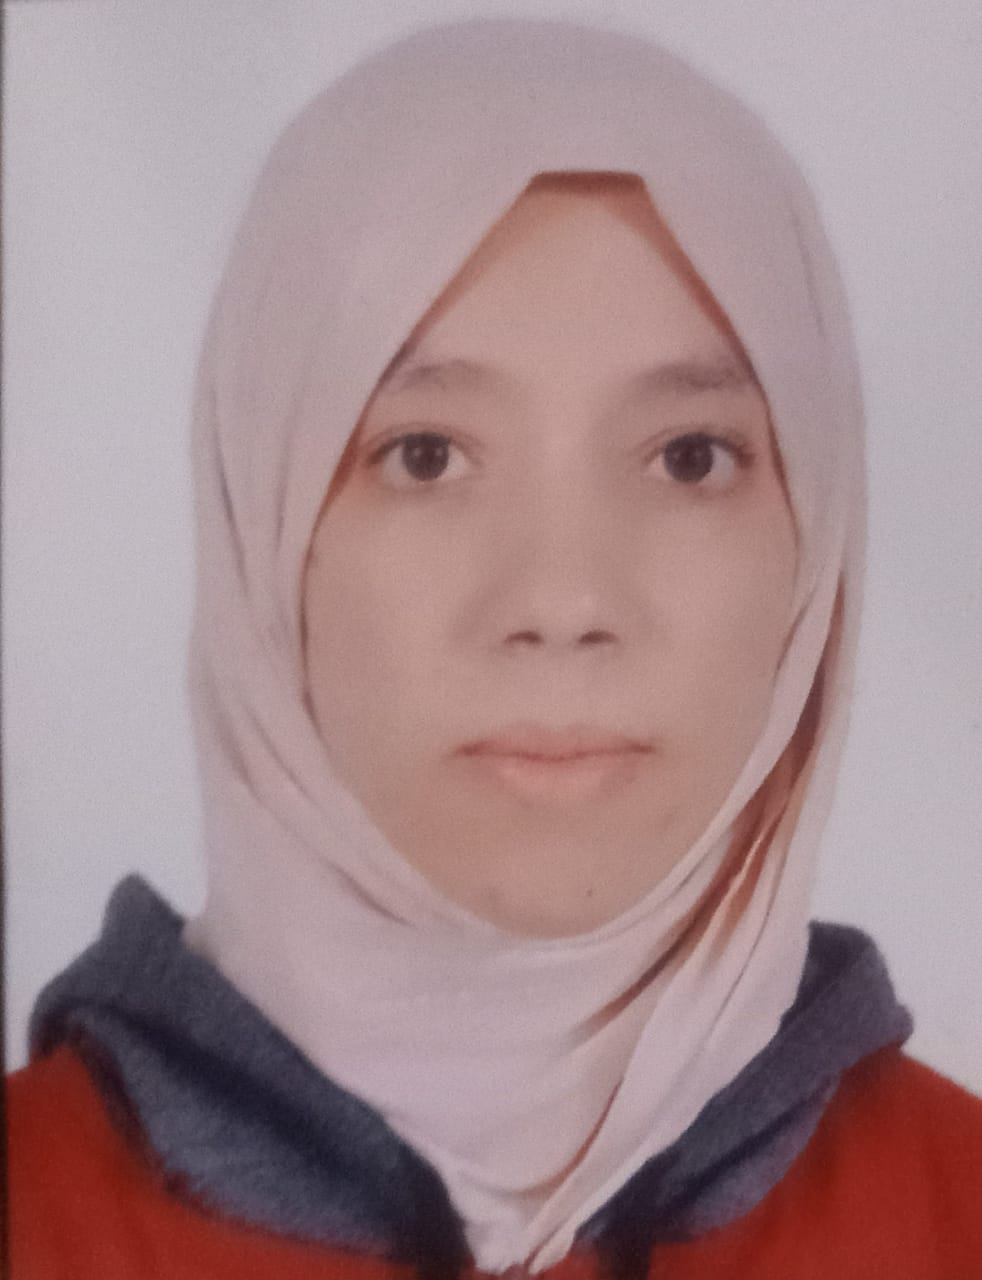
\includegraphics[width=0.5\linewidth]{WhatsApp Image 2021-09-07 at 10.33.40}	%trimming relative to image size
\end{center}

%---------------------------------------------------------------------------------------
%	META SKILLS
%----------------------------------------------------------------------------------------


\cvsection{CONTACT}

\icontext{MapMarker}{12} {802 hay salam Ouarzazate \\ Maroc}{black}\\[6pt]
\icontext{MobilePhone}{12}{	06 96 50 60 08}{black}\\[6pt]
\iconemail{Envelope}{12}{amalezzaki82@gmail.com}{amalezzaki82@gmail.com}{black}\\[6pt]




\cvsection{LANGUES}

\cvskill{Français} {} {0.6} \\[-2pt]

\cvskill{Anglais} {} {0.8} \\[-2pt]

\cvskill{Arabe} {} {1} \\[-2pt]







%---------------------------------------------------------------------------------------
%	EDUCATION
%----------------------------------------------------------------------------------------


%---------------------------------------------------------------------------------------
%	CERTIFICATION
%----------------------------------------------------------------------------------------

\end{leftcolumn}
\begin{rightcolumn}
%---------------------------------------------------------------------------------------
%	TITLE  HEADER
%----------------------------------------------------------------------------------------
\fcolorbox{white}{darkcol}{\begin{minipage}[c][3.5cm][c]{1\mpwidth}
	\begin {center}
		\HUGE{ \textbf{ \textcolor{white}{ \uppercase{ AMAL EZZAKI } } } } \\[-24pt]
		\textcolor{white}{ \rule{0.1\textwidth}{1.25pt} } \\
		
	\end {center}
\end{minipage}} \\[14pt]
\vspace{-12pt}

%---------------------------------------------------------------------------------------
%	PROFILE
%----------------------------------------------------------------------------------------

 

%---------------------------------------------------------------------------------------
%	WORK EXPERIENCE
%----------------------------------------------------------------------------------------
 
\cvsection{Education}


\cvevent
{2013}
{Formation préparatoire pour les cadres du camp d'été}
{Direction Régionale des affaires de la jeunesse, de l'enfance et de la femme Ouarzazate}
{}

{\cvlist{
		\item Creation of a web portal for role- and rights management
		\item Establishing a connection to the existing MicroFocus role solution
		\item Development of new role-based workfows and processes, as well as training and support
		\item Maintenance of existing infrastructure
}}
{\cvlist{
		\item Creation of a web portal for role- and rights management
		\item Establishing a connection to the existing MicroFocus role solution
		\item Development of new role-based workfows and processes, as well as training and support
		\item Maintenance of existing infrastructure
}}
{}



\vspace{7pt}

\cvevent
{2018}
{Diplôme du formation spécialité : Opérateur de Saisie
}
{Centre de formation par apprentissage El Moukawama Ouarzazate}
{}
{}
{\cvlist{
		\item A web based tool for an intuitive role assignment and administration
		\item Online overview of company structures, projects, etc
		\item Tools for role review, reporting and troubleshooting
}}


\vspace{7pt}
\cvevent
{2013- 2015}
{Licence professionnelle : filière : English Studies ; Communication
	and pedagogy
}
{faculté polydisciplinaire ouarzazate}
{}
{}
{\cvlist {
		\item Django for the roles- and rights management tool backend (backend is a REST interface)
		\item Angular for the easy frontend interaction
		\item HTML5/CSS3/Bootstrap3 for the frontend
		\item Ansible + Docker for 1-click deployments
}}
{\cvlist{
		\item A dddddd based tool for an intuitive role assignment and administration
		\item Online overview of company structures, projects, etc
		\item Tools for role review, reporting and troubleshooting
}}

 

\vspace{7pt}


\cvevent
{2012 - 2013
	}
	{Baccalauréat en Lettres et Sciences humaines : option LETTRES}
	{Lycée Sidi daoud Ouarzaate}
	{}
	{}
	{\cvlist{
			\item Creation of a web portal for role- and rights management
			\item Establishing a connection to the existing MicroFocus role solution
			\item Development of new role-based workfows and processes, as well as training and support
			\item Maintenance of existing infrastructure
	}}
	{\cvlist {
			\item Django for the roles- and rights management tool backend (backend is a REST interface)
			\item Angular for the easy frontend interaction
			\item HTML5/CSS3/Bootstrap3 for the frontend
			\item Ansible + Docker for 1-click deployments
	}}
 
	
 
 \vspace{7pt}

\cvsection{EXPÉRIENCES PROFESSIONELLES}

\cvevent
{2016
}
{stagiaire en enseignement d'anglais }
{Collége Abderahim Bouabid Ouarzazate}
{}
{}
{\cvlist{
		\item Creation of a web portal for role- and rights management
		\item Establishing a connection to the existing MicroFocus role solution
		\item Development of new role-based workfows and processes, as well as training and support
		\item Maintenance of existing infrastructure
}}
{\cvlist {
		\item
		Création de plans de cours conformément au programme scolaire de l'État et aux normes du programme scolaire de collége.
			\item	
		Collaborer avec d'autres membres du personnel pour planifier et programmer des leçons favorisant l'apprentissage et l'engagement des élèves.
				\item
		Gérer des classes de 30 élèves pendant l'absence des enseignants désignés. 
}}
{\cvlist {
		\item
		Création de plans de cours conformément au programme scolaire de l'État et aux normes du programme scolaire de collége.
		\item	
		Collaborer avec d'autres membres du personnel pour planifier et programmer des leçons favorisant l'apprentissage et l'engagement des élèves.
		\item
		Gérer des classes de 30 élèves pendant l'absence des enseignants désignés. 
}}

\vspace{7pt}

\cvevent
{2015
}
{Entraîneur de camp d'été }
{Association Camps Urbains Ouarzazate}
{}
{}
{\cvlist{
		\item Creation of a web portal for role- and rights management
		\item Establishing a connection to the existing MicroFocus role solution
		\item Development of new role-based workfows and processes, as well as training and support
		\item Maintenance of existing infrastructure
}}
{\cvlist {
	\item Créer une atmosphère éducative qui offrirait à l'enfant bénéficiaire un terrain fertile pour la formation d'une personnalité de la manière la plus correcte
\item 	Diriger les tendances de l'enfant et affiner son talent, par l'autonomie	
\item T	Préparer un ensemble d'activités utiles sur le plan éducatif, culturel, artistique et sportif
}}
{\cvlist {
		\item Créer une atmosphère éducative qui offrirait à l'enfant bénéficiaire un terrain fertile pour la formation d'une personnalité de la manière la plus correcte
		\item 	Diriger les tendances de l'enfant et affiner son talent, par l'autonomie	
		\item Préparer un ensemble d'activités utiles sur le plan éducatif, culturel, artistique et sportif
}}


\vspace{7pt}
\cvsection{Compétences}


\textbf{Soft Skills} : Le leadership - Bonne capacité de communication - Travail d'équipe - Résolution de problèmes - 
Intelligence sociale et émotionnelle -Compétence culturelle
\\
\textbf{informatique bureautique} : Word - Excel 


\end{rightcolumn}
\end{paracol}
\end{document}
